\chapter{Second-Order System Identification and Analysis}\label{Lab:2}
A large majority of systems we wish to control are physical systems. These
systems are often modelled using Newton's laws
\[
\begin{aligned}
  \mathrm{mass}~\frac{\mathrm d^2}{\mathrm{d}t^2}~\mathrm{position}
    &= \sum \mathrm{natural~forces} + \mathrm{applied~force},\\
  \mathrm{inertia}~\frac{\mathrm d^2}{\mathrm{d}t^2}~\mathrm{orientation}
    &= \sum \mathrm{natural~torques} + \mathrm{applied~torque},
\end{aligned}
\]
These systems --- when
they are linear --- result in second-order transfer functions from the
applied input (forces or torques) to the output (position and orientation).
It follows that if we want to understand how to effectively control physical
systems then we must first understand second-order systems and their
properties!

In this lab you will explore the generic characteristics of a second-order
linear system. You will discover the limitations of proportional error
feedback control --- the most na\'ive of control laws --- when applied to
a physical system. This motivates consideration of
more complicated control strategies. Labs 4 and 5 will explore these options.

\emph{A word of caution. This is the final lab where it is possible to
to find out the parameters of your system by inspecting the data file.
This, in principal, allows you to back-calculate what your procedures should
tell you. This was intentional to allow
you to check your work and ensure you understand how to perform the procedure.
However, future labs will assume you've perfected this procedure.
The parameters will be fairly well hidden like how it is sometimes in the
\texttt{\#RealWorld}. So, make sure you understand how to perform the
procedures!}

\section{Objectives}
The primary objectives of this lab are to
\begin{enumerate}[label=(\arabic*)]
  \item{
    \textbf{Learn} the characteristic properties of a standard second-order linear system.
  }
  \item{
    \textbf{Identify} the parameters of a standard second-order linear system.
  }
  \item{
    \textbf{Learn} how to acquire a Bode plot, the frequency response,
    and \textbf{understand} how to interpret it.
  }
  \item{
    \textbf{Explore} how a proportional control feedback affects the response
    of a second-order system.
  }
\end{enumerate}
Below is a dependency graph depicting the relationships between each of the
deliverables. If an arrow flows from A to B, that means B depends on the
partial or full completion of A.
\begin{center}
\begin{tikzpicture}[x=1em, y=1em]
  \node[deliverable] (D_2_1) {Deliverable\\\ref{lab2:d1}};
  \node[deliverable, below = 3em of D_2_1] (D_2_3) {%
    Deliverable\\\ref{lab2:d2b}%
  };
  \node[deliverable, right = 3em of D_2_3] (D_2_2) {%
    Deliverable\\\ref{lab2:d2}%
  };
  \node[deliverable, right = 3em of D_2_2] (D_2_7_4) {%
    Deliverable\\\ref{lab2:report}~\ref{lab2:report:q4}-\ref{lab2:report:q4b}%
  };
  \node[deliverable, at=(D_2_1-|D_2_7_4)] (D_2_7_1) {%
    Deliverable\\\ref{lab2:report}~\ref{lab2:report:q1}--\ref{lab2:report:q3}%
  };

  \node[deliverable, below = 3em of D_2_3] (D_2_4) {%
    Deliverable\\\ref{lab2:d3a}%
  };
  \node[deliverable, at = (D_2_4-|D_2_7_4)] (D_2_7_6) {%
    Deliverable\\\ref{lab2:report}~\ref{lab2:report:q5}%
  };
  \node[deliverable, below = 3em of D_2_4] (D_2_5) {%
    Deliverable\\\ref{lab2:d3}%
  };
  \node[deliverable, right = 6em of D_2_5] (D_2_6) {%
    Deliverable\\\ref{lab2:d4}%
  };
  \node[deliverable, right = 6em of D_2_6] (D_2_7_7) {%
    Deliverable\\\ref{lab2:report}~\ref{lab2:report:q6}%
  };
  \node[deliverable, below = 3em of D_2_7_7] (D_2_7_8) {%
    Deliverable\\\ref{lab2:report}~\ref{lab2:report:q8}%
  };


%  \draw[signal, arrow] (D_2_1.south) -- (D_2_3.north);
  \draw[signal, arrow] (D_2_1.east) -- (D_2_7_1.west);
  \draw[signal, arrow] (D_2_3.east) -- (D_2_2.west);
  \draw[signal, arrow] (D_2_2.east) -- (D_2_7_4.west);
  \draw[signal, arrow] (D_2_7_1.south) -- (D_2_7_4.north);
  \draw[signal, arrow] (D_2_4.east) -- (D_2_7_6.west);
  \draw[signal, arrow] (D_2_5.east) -- (D_2_6.west);
  \draw[signal, arrow] (D_2_5.east) -- (D_2_7_6.west);
  \draw[signal, arrow] (D_2_6.east) -- (D_2_7_7.west);

\end{tikzpicture}
\end{center}

\section{Experimental Procedure}
This entire lab will be done using the ``\texttt{Lab\_2.slx}'' Simulink model.
In there you will
find a number of blocks already placed for you in an open loop configuration:
\begin{itemize}
  \item{a step input,}
  \item{a summing junction,}
  \item{an adjustable gain block,}
  \item{a ``fill-in'', zero disturbance block,}
  \item{a ``plant'', the system we are going to analyze, and}
  \item{a terminator.}
\end{itemize}
This time we will \emph{not} use the signal generator and instead leverage
the Model Linearizer App. Its usage is described in Appendix
\ref{App:Simulink:ModelLinearizer}. You may acquire the step response
using the techniques described in Lab~\ref{Lab:1} but to acquire the frequency
response you will have to use the Model Linearizer app. In future, we will
primarily rely on the Model Linearizer app as it'll
unify all your data collection
requirements and is far easier to use than modifying a script and turning
on/off logging. For this lab, the input signal starts off configured
as \(r\) and the output signal as \(y.\) You will have to change it later
in the lab.
%
The plant --- labelled \(P(s)\) in the Simulink diagram --- can be assumed
to be a transfer function taking the form
\[
  P(s) = \frac{\hat{K}\omega_n^2}{s^2 + 2\zeta\omega_n s + \omega_n^2}.
\]
This form has a special name.
%
\begin{definition}[]{Standard Second-Order Form}
  The standard second-order order form for a strictly proper, second-order
  transfer function \(P(s)\) with no zero is
  \[
    P(s) = \frac{\hat{K} \omega^2}{s^2 + 2 \zeta \omega s + \omega^2}.
  \]
  where \(\omega\) is called the \textbf{natural frequency} and
  \(\zeta\) is the \textbf{damping ratio}.
\end{definition}
%
The primary goal of this experiment is to (1) estimate \(\zeta,\)\(\omega_n,\)
and \(\hat{K},\) (2) explore the characteristics of your system and
(3) see how the characteristics change under a proportional error controller.
When analyzing the \emph{closed loop system}, we put our system in the form
depicted by Figure~\ref{fig:lab2:closing-loop}.
%
\begin{figure}
  \centering
  \begin{tikzpicture}[x=1in, y=1in]
    \node [draw, block] (Controller) {\(K_p\)};
    \node [draw, block, right=0.5 of Controller] (Plant) {\(P(s)\)};
    \node [draw, summer, left=0.5 of Controller] (Sum) {};
    \node [draw, summer, right=0.5 of Plant] (DistSum) {};
    \node [above=0.5 of DistSum] (AboveDistSum) {};
    \node [below=0.5 of Sum] (BelowSum) {};

    \draw [arrow, signal]
      (AboveDistSum.base)
      --
      (DistSum.north)
      node [above right, annotate] {\(d\)};
    \draw [arrow, signal]
      (Controller.east) -- (Plant.west)
      node [below left, annotate] {\(u\)};
    \draw [arrow, signal]
      (Plant.east)
      --
      (DistSum.west)
      node [below left, annotate] {\(+\)};
    \draw [arrow, signal]
      (DistSum.east)
      --
      +(0.5, 0)
      |-
      (BelowSum.base)
      --
      (Sum.south)
      node [below right, annotate] {\(-\)};
    \draw [arrow, signal]
      (Sum.east) -- (Controller.west);
    \draw [arrow, signal]
      ($(Sum.west)+1*(-0.5, 0)$) -- (Sum.west)
      node [below left, annotate] {\(r\)};
    \draw [arrow, signal]
      (DistSum.east) -- +(1, 0)
      node [below, annotate] {\(y\)};
  \end{tikzpicture}
  \caption{
    Closing the loop around the Plant \(P(s)\) for Lab 2. Note that the
    loop is closed \emph{after} the disturbance has been added to the output.
  }
  \label{fig:lab2:closing-loop}
\end{figure}
%

\subsection{Measuring the Characteristics of a Second Order System}
In Lab~\ref{Lab:1}, you learned about the DC gain, the bandwidth, and
settling time of a first-order system.
We will use these characteristics, as well as one more new one, to help
characterize a second order plant.
%
Your deliverable for this section is
%
\begin{deliverable}[label={lab2:d1}]
  \textbf{Capture a figure} showing your system's open loop step response.
  \textbf{Measure} and \textbf{record}
  \begin{enumerate}[label=(\arabic*)]
    \item{the steady-state value \(y_{\mathrm{ss}},\)}
    \item{
      the time-to-peak value \(T_{\mathrm{peak}}\) and
      the peak value \(y_{\mathrm{max}},\) and
    }
    \item{
      the \(2\%\) settling time \(T_{\mathrm{s}}.\)
    }
  \end{enumerate}
  The figure included in your report must have \textbf{cursors} at the peak
  value and steady-state value.
\end{deliverable}
%
You are already familiar with most of these measurements. The new measurements
are the peak related measurements. For us, the following definition suffices.
%
\begin{definition}[]{Time-To-Peak and Overshoot}
  Let \(G(s)\) be a proper, stable transfer function
  that maps an input signal \(u(t)\) to an output \(y(t).\)
%
  Let \(u(t)\) be the (not necessarily unit) step function. The peak value
  of \(y(t)\) is the maximum value \(y(t)\) obtains, mathematically expressed
  by\footnote{normally \(\sup\) is used but this suffices for our purposes.}
  \[
    y_\mathrm{max} \defineas \max_{\tau \in \Real} \left| y(\tau) \right|
  \]
  and the time it obtains the peak value, known as \textbf{time-to-peak}
  is defined as
  \[
    T_\mathrm{peak} \defineas \argmax_{\tau \in \Real} \left| y(\tau) \right|.
  \]
  Then, if \(y_\mathrm{ss}\) is the steady-state value of \(y(t),\) the
  \textbf{percent overshoot} is defined as
  \[
    \%\mathrm{OS}
      \defineas
        \frac{%
          \left|
            \left|y_\mathrm{max}\right| - \left|y_\mathrm{ss}\right|
          \right|%
        }{%
          \left| y_\mathrm{ss}\right|%
        }.
  \]
\end{definition}
%
Figure~\ref{fig:lab2:peak} depicts the measurements you perform to acquire
the percent overshoot. You measure the maximum value of the output
signal and the steady-state value of the signal. Then you
compute the relative error between the maximum value and the settling value of
the output.
%
\begin{figure}
  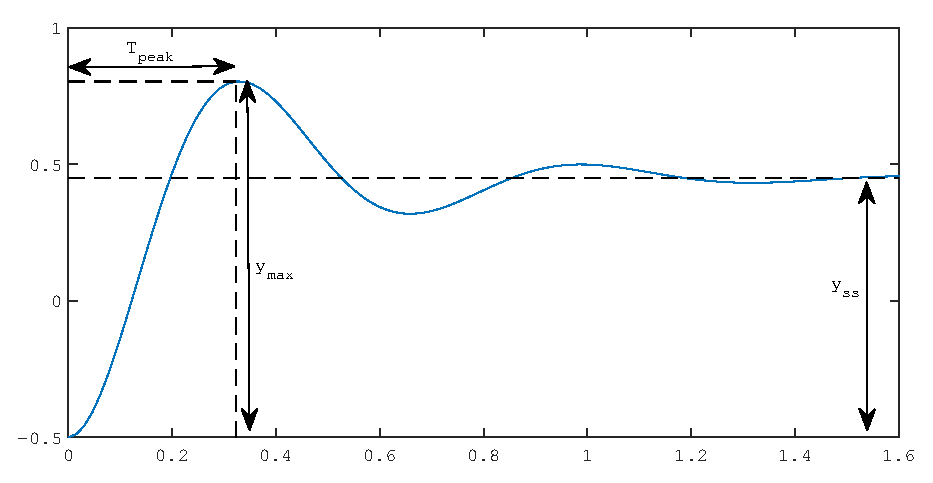
\includegraphics{images/Lab_2_Peak.eps}
  \caption[Depicting Overshoot Measurements for a Second-Order System.]{%
    The maximum peak occurs at time \(T_\mathrm{peak}\) with amplitude
    \(y_\mathrm{max}.\) The steady-state value is shown as \(y_{\mathrm{ss}}.\)
  }
  \label{fig:lab2:peak}
\end{figure}
%
\begin{procedure}[label={proc:lab2:p1}]
  In this procedure you will capture a variety of characteristics of
  your provided second-order system to achieve the goal of Deliverable
  \ref{lab2:d1} and to eventually characterize the parameters \(a,\)\(b\)
  and \(K.\)
  \begin{enumerate}[label=(\arabic*)]
    \item{
      \textbf{Ensure} your system is in the open loop configuration.
    }
    \item{
      \textbf{Ensure} that you indicate the signal before the summing junction
      is an input signal (Input Perturbation) and the signal after the plant
      is indicated as an output signal (Output Measurement). Refer
      to Appendix~\ref{App:Simulink:ModelLinearizer:2} for more information
      on how to do so.
    }
    \item{
      \textbf{Open} the Model Linearizer app and \textbf{capture} a
      step response. Refer to Appendix~\ref{App:Simulink:ModelLinearizer:3}
      on how to do so.
    }
    \item{
      \textbf{Measure} and \textbf{record} the following parameters of the
      output signal:
      \begin{itemize}
        \item{
          the steady-state value \(y_{\mathrm{ss}},\)
        }
        \item{
          the time-to-peak value \(T_{\mathrm{peak}}\) and
          the peak value \(y_{\mathrm{max}},\)
        }
        \item{
          the \(2\%\) settling time \(T_{\mathrm{s}}.\)
        }
      \end{itemize}
      \label{proc:lab2:p1:4}
    }
  \end{enumerate}
\end{procedure}

\subsection{Exploring Proportional Error Feeedback}
For this section you will explore how proportional error feedback affects
the behaviour of a second-order system. You will complete the following
deliverables.
%
\begin{deliverable}[label={lab2:d2}]
  \textbf{Capture} a single step response of your closed-loop system
  with a gain \(K_p \neq 1.\)
\end{deliverable}
%
\begin{deliverable}[label={lab2:d2b}]
  \textbf{Fill} three rows of the table
  \begin{center}
  \begin{tabular}{c|c|c|c|c}
    \(K_p\)
      & \(y_\mathrm{ss}\)
      & \(y_\mathrm{max}\)
      & \(T_\mathrm{peak}\)
      & \(\%\mathrm{OS}\) \\
    Gain
      & Steady-State Value
      & Peak Value
      & Time-To-Peak
      & Overshoot \\ \hline
    \(1\) & & & & \\ \hline
    Any & & & & \\ \hline
    Any & & & & \\ \hline
    & & & &
  \end{tabular}
  \end{center}
  for the closed loop system.
  Note that the overshoot is computed from \(y_\mathrm{ss}\) and
  \(y_\mathrm{max}.\)
\end{deliverable}

%
\begin{procedure}[label={proc:lab2:p2}]
  In this procedure you will explore a variety of gains \(K_p.\)
  \begin{enumerate}[label=(\arabic*)]
    \item{
      \textbf{Ensure} your system is in the closed-loop configuration
      as depicted in Figure~\ref{fig:lab2:closing-loop}.
    }
    \item{
      Choose a sequence of three gains to test. One of these gains
      must be \(K_p = 1.\) You may choose any value that is allowed by
      the slider gain provided to you in the Simulink Diagram.
    }
    \item{
      For each of your chosen gains \(K_p,\) \textbf{compute} the step
      response and \textbf{fill} the relevant row of the table
      in Deliverable~\ref{lab2:d2b}
    }
  \end{enumerate}
\end{procedure}

\subsection{Acquiring the Bandwidth in the Frequency-Domain}
Once again we will acquire the bandwidth of our system. We will do so for
\emph{both} the closed and open loop configurations. This time, however,
we will do so using the frequency response. In particular, you are asked
to complete the following deliverables.
%
\begin{deliverable}[label={lab2:d3a}]
  \textbf{Capture} a figure of the Bode plot for the open loop system.
  \textbf{Include} a cursor at the bandwidth frequency on the magnitude
  plot and a cursor where you estimated the DC gain.
\end{deliverable}
%
\begin{deliverable}[label={lab2:d3}]
  \textbf{Capture} a figure of the Bode plot for the closed loop system
  with unity gain (\(K_p = 1\)).
  \textbf{Include} a cursor at the bandwidth frequency on the magnitude
  plot.
\end{deliverable}
%
First of all, let us briefly review what a Bode plot depicts.
Given a \emph{real, rational and stable} transfer function \(G(s)\) and
(co)sinusoidal input
\(U(s) = \frac{s}{s^2 +\omega^2}\) of frequency \(\omega,\) the
output \(y(t)\) converges towards the signal
\[
  y_\mathrm{ss}(t)
    = \left\| G(j\omega) \right\| \cos(\omega t + \measuredangle G(j\omega)).
\]
Sometimes we say that the signal \(y_\mathrm{ss}(t)\) is the output of
\(G(s)\) in \emph{steady state}.
Recognizing that the input was \(u(t) = \cos(\omega t),\) we observe that the
output in steady state is an amplified/attenuated and phase shifted
version of the input.

The amplification or attenuation of the signal \(u(t)\) is determined by
\(\left\|G(j\omega)\right\|.\) This is what is plotted in the \textbf{
Magnitude Plot} of a Bode plot. Normally the standard units of this
multiplicative factor is decibels, i.e.
\[
\left\|G(j\omega)\right\|_{\mathrm{dB}} = 20 \log_{10}\left( \left\|G(j\omega)\right\| \right).
\]
Remember when reading a Bode plot, such as in MATLAB, you will often have to
convert from the decibel value \(\left\|G(j\omega)\right\|_{\mathrm{dB}}\) on
the left to the unitless magnitude \(\left\|G(j\omega)\right\|\) on the right.
We will not concern ourselves with the phase plot in this lab but normally
the units of the phase shift is degrees.

The magnitude plot can be used to measure the DC gain and bandwidth frequency.
You will recall from Lab~\ref{Lab:1} that the DC gain can be approximated by
the gain of \(G(s)\) at low sinusoidal frequencies. This amounts to looking
at the value that \(\left\| G(j\omega) \right\|\) tends towards as
\(\omega\to 0.\)
%
Further you will recall from Definition~\ref{def:bandwidth} that the
bandwidth frequency \(\omega_\mathrm{bw}\) of \(G(s)\) solves the
equation
\[
  \frac{1}{\sqrt{2}} = \frac{\left\|G(j\omega_\mathrm{bw})\right\|}{\left\|G(0)\right\|}.
\]
Converting our expression to be in decibels yields the approximate relation
\[
  \left\| G(j\omega_\mathrm{bw}) \right\|_{dB} = \left\|G(0)\right\|_{dB} - \SI{3}{dB}.
\]
This suggests that to measure the bandwidth frequency, it suffices to look
for the point where the magnitude plot \(\left\|G(j\omega)\right\|_{dB}\)
crosses the value \(\SI{3}{dB}\) below the DC gain
\(\left\|G(0)\right\|_{dB}.\)

%
\begin{procedure}[label={proc:lab2:p3}]
  \begin{enumerate}[label=(\arabic*)]
    \item{
      \textbf{Ensure} your system is in the open-loop configuration.
      \textbf{Ensure} the gain \(K_p\) is set to \(1.\)
    }
    \item{
      \textbf{Open} the Model Linearizer App.
    }
    \item{
      \textbf{Acquire} a Bode plot. Your Bode plot will probably look a lot
      like Figure~\ref{fig:lab2:bode}. Note that, for some of you, you may
      have a little peak in the magnitude plot like in
      Figure~\ref{fig:lab2:bode:b}; this is normal!
      \label{proc:lab2:p3:3}
    }
    \item{
      \textbf{Measure} the DC gain on the Magnitude plot using a cursor.
      The DC gain is the value that the Magnitude Plot tends to
      as \(\omega \to 0.\)
    }
    \item{
      \textbf{Measure} the frequency \(\omega\) at which the gain
      (magnitude plot) drops to a value \(\SI{3}{dB}\)
      below the DC gain measured in the previous step. This frequency
      is called the \textbf{bandwidth}.
      \label{proc:lab2:p3:5}
    }
  \end{enumerate}
\end{procedure}
%
\begin{procedure}[label={proc:lab2:p4}]
  \begin{enumerate}[label=(\arabic*)]
    \item{
      \textbf{Put} your system is in the closed-loop configuration as
      depicted by Figure~\ref{fig:lab2:closing-loop}.
      \textbf{Ensure} the gain \(K_p\) is set to \(1.\)
    }
    \item{
      Repeat steps~\ref{proc:lab2:p3:3}--\ref{proc:lab2:p3:5} of
      Procedure~\ref{proc:lab2:p3}.
      %\emph{Did you know you can overlay
      %this Bode plot on top of the Bode plot of Procedure~\ref{proc:lab2:p3}?
      %This is not required, but you can do so if you like.
      %To do so, take the Bode plot of the open loop system. Then, change the
      %configuration. Finally, instead of pressing ``\texttt{Bode Plot}'' press
      %a new button with the title of the plot. In my case it was
      %``\texttt{Bode Plot 1}.'' You will have something replicating that of
      %Figure~\ref{fig:lab2:bodeclosed}}
    }
  \end{enumerate}
\end{procedure}
%
\begin{figure}
  \centering
  \subfloat[A fairly well damped second order system.]{%
    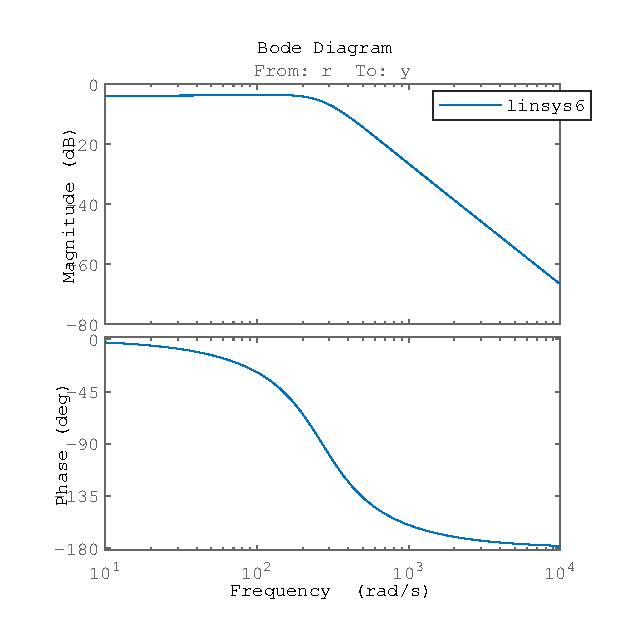
\includegraphics{images/Lab_2_Bode.eps}%
  }\hfill\\
  \subfloat[A much less damped, \(\zeta << 0.707,\) second order system.%
  \label{fig:lab2:bode:b}]{%
    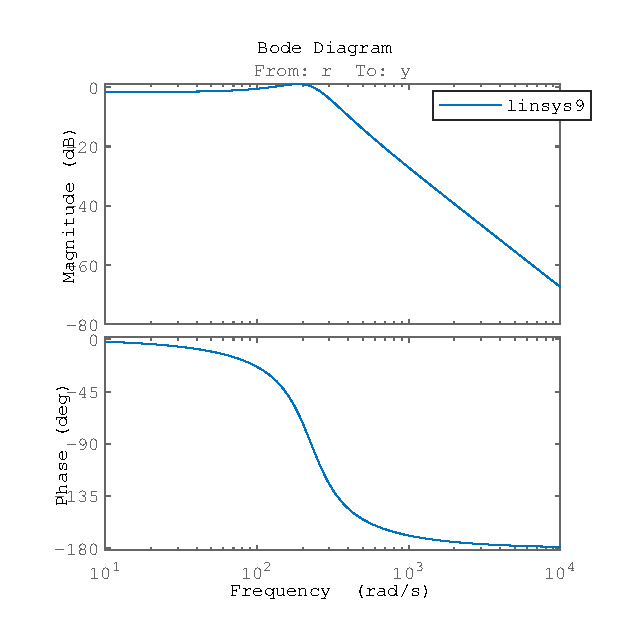
\includegraphics{images/Lab_2_Bode_Peak.eps}%
  }\hfill\\
  \caption[Sample Bode Plots of a Second Order System]{
    Sample Bode plots of a second order system.
  }
  \label{fig:lab2:bode}
\end{figure}
%
% \begin{figure}
%   \centering
%   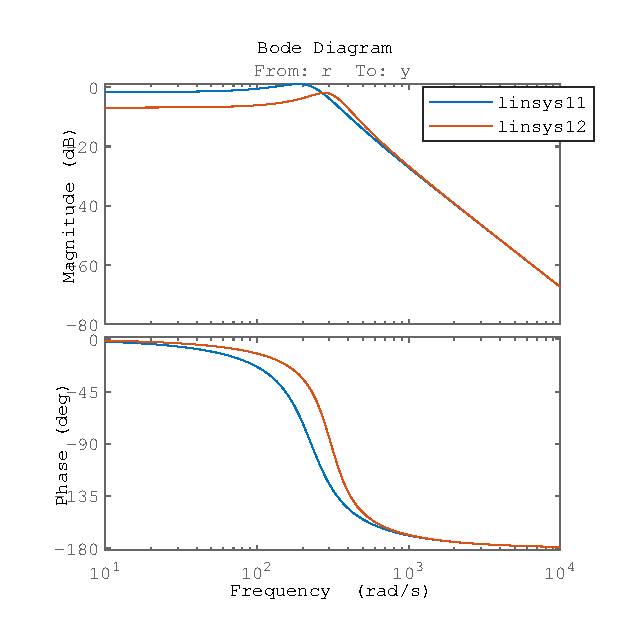
\includegraphics{images/Lab_2_Bode_ClosedLoop.eps}%
%   \caption[Sample Overlayed Bode Plots of a Second Order System]{
%     Sample overlayed Bode plots of a second order system.
%   }
%   \label{fig:lab2:bodeclosed}
% \end{figure}
%

\subsection{Disturbance Rejection}
You have almost completed the experimental part of this lab. This section
explores how the closed-loop affects disturbance rejection. Disturbances are
signals that we haven't modelled \emph{or} cannot be modelled and therefore
cannot account for. Naturally, large enough disturbances affect our ability to
control systems. The beauty of control is that we can design systems that
mitigate disturbances we do not explicitly model or know about! Here we will
find that our system can mitigate some types of disturbance signals, but not
all. The only deliverable for this section is
%
\begin{deliverable}[label={lab2:d4}]
  \textbf{Include} a Bode plot illustrating the response from the
  \emph{disturbance input signal} \(d(t)\) to the output signal \(y(t).\)
  \textbf{Include} a cursor on the magnitude plot at \emph{the bandwidth
  frequency of the closed loop system.} (The frequency found in
  Deliverable~\ref{lab2:d3})
\end{deliverable}
%
To fulfill this deliverable, you must acquire a Bode plot of the input to
output relationship between \(d\) and \(y.\)
%
\begin{procedure}[label={proc:lab2:p5}]
  For this procedure, you will change the input signal. You will remove the
  ``\texttt{Input Perturbation}'' annotation from the reference \(r\) and
  place it on the disturbance \(d.\)

  \begin{enumerate}[label=(\arabic*)]
    \item{
      \textbf{Ensure} the system is in the closed-loop configuration
      depicted in Figure~\ref{fig:lab2:closing-loop}.
      \textbf{Set} the gain \(K_p\) to \(1.\)
    }
    \item{
      \textbf{Remove} the ``\texttt{Input Perturbation}'' annotation from
      the reference signal. This amounts to repeating the process described
      in Appendix~\ref{App:Simulink:ModelLinearizer:2}, i.e. right click the
      signal wire \(r\) and press
      \texttt{Linear Analysis Points/Input Perturbation} so that the
      input perturbation icon disappears from the signal wire \(r.\)
    }
    \item{
      \textbf{Add} the ``\texttt{Input Perturbation}'' annotation to the
      the disturbance signal wire \(d.\)
    }
    \item{
      \textbf{Open} the Model Linearizer App and \textbf{acquire} a Bode
      plot. \emph{Expect the Bode plot to look substantially different than
      your previous Bode plots.}
    }
  \end{enumerate}
\end{procedure}

\section{Report Deliverable}
Good job! You made it through Lab~\ref{Lab:2}.
You are required to submit a report
that verifies you completed Lab~\ref{Lab:2} and that demonstrates you
understand the procedures you performed. In addition to including
\begin{itemize}
  \item{Deliverable~\ref{lab2:d1},}
  \item{Deliverable~\ref{lab2:d2},}
  \item{Deliverable~\ref{lab2:d2b},}
  \item{Deliverable~\ref{lab2:d3a},}
  \item{Deliverable~\ref{lab2:d3} and }
  \item{Deliverable~\ref{lab2:d4}}
\end{itemize}
in your report,
you are required to answer the questions of the following deliverable.
Make sure to leverage your other deliverables in your answers!
\begin{deliverable}[label={lab2:report}]
  \begin{enumerate}[label={(\arabic*)}]
    \item{
      Using the characteristics collected in Step~\ref{proc:lab2:p1:4} of
      Procedure~\ref{proc:lab2:p1}, \textbf{determine} the parameters
      \(\hat{K},\) \(\omega_n\) and \(\zeta\) that describe your plant \(P(s)\)
      in the standard second order form
      \[
        P(s) = \frac{\hat{K} \omega_n^2}{s^2 + 2 \zeta \omega_n s + \omega_n^2}
        .
      \]
      \emph{Notes: This time you drove the system with a unit
      step input. As a result, the steady-state value \(y_\mathrm{ss}\)
      is equal to the DC gain \(\hat{K}.\) The \(2\%\) settling time for a
      underdamped, standard second order system is approximated by the expression
      \[
        T_{2\%} \approx \frac{4}{\zeta \omega_n}
      \]
      and the percent overshoot is given by the formula
      \[
        \%\mathrm{OS} = 100 e^{\left(
          \frac{-\zeta \pi}{\sqrt{1-\zeta^2}}
        \right)}.
      \]
      So you should be able to solve for \(\hat{K}\) and \(\zeta\) first, then
      use them to solve for \(\omega_n.\)
      }
      \label{lab2:report:q1}
    }
    \item{
      It can be shown that the time-to-peak, another measurement you
      acquired, is equal to
      \[
        T_p = \frac{\pi}{\omega_n \sqrt{1-\zeta^2}}.
      \]
      Using your already acquired estimate of \(\zeta,\) \textbf{estimate}
      \(\omega_n\) using the time-to-peak.
      Based on your estimates, \textbf{explain} which you would rather use to
      estimate \(\omega_n:\) the time-to-peak or the \(2\%\) settling time.
      \label{lab2:report:q2}
    }
    \item{
      For the closed-loop diagram of Figure~\ref{fig:lab2:closing-loop},
      \textbf{compute} the transfer function from \(r\) to \(y.\)
      \textbf{Compute} the damping ratio, DC gain, and natural frequency of the
      closed-loop second-order system in terms of your plant's
      \(\hat{K},\) \(\omega_n\) and \(\zeta.\)
      \label{lab2:report:q3}
    }
    % \item{
    %   Given the open-loop damping ratio and natural frequency found in
    %   \ref{lab2:report:q1} and closed-loop damping ratio and natural
    %   frequency derived in~\ref{lab2:report:q2},
    %   \textbf{discuss} how closing the loop with unity feeback (\(K_p = 1\))
    %   affects the damping ratio and natural frequency of the
    %   second order system.
    %   \label{lab2:report:q3}
    % }
    \item{
      Using the table filled out in Deliverable~\ref{lab2:d2b} and the
      formulas you derived in~\ref{lab2:report:q2},
      \textbf{discuss} how changing the
      gain \(K_p\) affects the steady-state value \(y_\mathrm{ss},\) the
      time-to-peak \(T_p\) and the percent overshoot \(\%\mathrm{OS}.\)
      of the closed-loop second order step response.
      Also \textbf{discuss} how the settling time theoretically changes in the
      closed loop as a function of \(K_p\) using the estimate formula shown in
      \ref{lab2:report:q1}.
      \emph{\textbf{Ensure} you discuss every characteristic
      you've collected; if there is no trend, say so; if the trend is
      complicated (not simply linear in \(K_p\)), say so.}
      \label{lab2:report:q4}
    }
    \item{
      By leveraging your answer for~\ref{lab2:report:q4}, \textbf{explain} why
      proportional error feedback control may not always be sufficient to
      control a physical system.
      \label{lab2:report:q4b}
    }
    \item{
      Using the bandwidth frequencies found in Procedures~\ref{proc:lab2:p3}
      and~\ref{proc:lab2:p4}, \textbf{state} how closing the loop
      changed the bandwidth frequency.
      \label{lab2:report:q5}
    }
    % \item{
    %   \textbf{Why} is it desireable to be able to change the bandwidth
    %   of a system?
    %   \label{lab2:report:q7}
    % }
    \item{
      Leveraging Deliverable~\ref{lab2:d4}, \textbf{discuss} how well the
      closed loop system rejects disturbance signals.
      \emph{Your answer should depend on the disturbance input frequency
      \(\omega\) and the closed loop bandwidth frequency which you marked
      on your plot.}
      \label{lab2:report:q6}
    }
    % \item{
    %   For the open-loop configuration, \textbf{derive} the transfer function
    %   from the disturbance signal \(d\) to the output \(y.\)
    %   \textbf{Compare} the disturbance rejection properties between the
    %   open-loop and closed-loop system.
    %   \label{lab2:report:q7}
    % }
    \item{
      \textbf{Derive} the closed-loop transfer function from the
      disturbance \(d\) to the output \(y.\) How do the disturbance rejection
      properties change as you increase \(K_p\)? Do they improve or degrade?
      \emph{You will receive full marks if you provide a theoretical
      justification. You will want to produce a transfer function from
      \(d\) to \(y\) and it will have the form
      \[
        \frac{s^2 + A s + B}{s^2 + A s + D}
      \]
      where \(A, B, D\) depend on the plant parameters and \(K_p.\)
      \(K_p\) should only appear in \(D.\) You can then split the
      above system into two subsystems
      \[
        \left[s^2 + A s + B\right]
        \left[\frac{1}{D}\frac{D}{s^2 + A s + D}\right]
      \]
      and recognize that \(K_p\) only affects the Bode plot of the latter
      system. This means it suffices to analyze the frequency response of
      \[
        \frac{1}{D}\frac{D}{s^2 + A s + D}
      \]
      as \(K_p\) varies. You can put this subsystem into standard second order
      form to aid in your analysis. You already should be able to argue how the
      DC gain and natural frequency of this new subsystem is affected by
      \(K_p,\) so it remains to connect this knowledge with how the Bode plot
      of this subsystem would be affected.}

      \emph{An empirical argument (showing the Bode plot for multiple \(K_p\))
      will receive at most half the marks.}

      \emph{A correct answer without proof of any sort will receive 1 mark.}
      \label{lab2:report:q8}
    }
  \end{enumerate}
\end{deliverable}

\subsection{Grading Scheme}
The grading scheme is shown in Table~\ref{tab:lab2:grading}. The breakdown of
your grade is shown per deliverable except in the case of the lab
questions where it is shown per question.
%
\begin{table}
\centering
\begin{tabular}{c|l|c}
        & Deliverable           & Marks  \\ \hline
        & \ref{lab2:d1}         & 5       \\ \hline
        & \ref{lab2:d2}         & 5       \\ \hline
        & \ref{lab2:d3a}        & 5       \\ \hline
        & \ref{lab2:d3}         & 5       \\ \hline
        & \ref{lab2:d4}         & 5       \\ \hhline{=|=|=}
Lab Subtotal&                       & 25      \\ \hhline{=|=|=}
        & \ref{lab2:report}~\ref{lab2:report:q1}  & 3       \\ \hline
        & \ref{lab2:report}~\ref{lab2:report:q2}  & 2       \\ \hline
        & \ref{lab2:report}~\ref{lab2:report:q3}  & 3       \\ \hline
        & \ref{lab2:report}~\ref{lab2:report:q4}  & 4       \\ \hline
        & \ref{lab2:report}~\ref{lab2:report:q4b} & 1       \\ \hline
        & \ref{lab2:report}~\ref{lab2:report:q5}  & 1      \\ \hline
        & \ref{lab2:report}~\ref{lab2:report:q6}  & 3      \\ \hline
        & \ref{lab2:report}~\ref{lab2:report:q8}  & 4       \\ \hhline{=|=|=}
Report Subtotal&  & 21 \\ \hhline{=|=|=}
  Total &                       & 46
\end{tabular}
\caption[Grading Scheme for Lab 2]{Grading scheme for Lab 2.}
\label{tab:lab2:grading}
\end{table}
%
